\documentclass[logo=EURECOM,english]{eurecombeamer}

\usepackage[utf8x]{inputenc}
\usepackage{cite}
\usepackage{graphicx}
\usepackage[font=scriptsize]{subfig}
\usepackage{tikz}
\usepackage{listings}
\usetikzlibrary{fadings}
\usepackage{tikz-uml}

\usepackage[binary-units, output-decimal-marker={,}]{siunitx}
\sisetup{
    output-decimal-marker=\text{,},
    detect-all=true,
    per-mode=fraction
}

\DeclareMathAlphabet{\mathbit}{OML}{cmr}{bx}{it}
\DeclareMathAlphabet{\mathsf}{OT1}{cmss}{m}{n}
\DeclareMathAlphabet{\mathbsf}{OT1}{cmss}{bx}{it}

\newcommand{\bcal}[1]{\boldsymbol{\cal #1}}
\newcommand{\brandom}{\mathbsf}
\newcommand{\random}{\mathsf}

\usepackage{minibox}

\renewcommand{\emph}[1]{\textcolor{EURECOMblue}{#1}}
\setbeamertemplate{bibliography item}[triangle]

\setbeamerfont{section in toc}{size=\scriptsize}
\setbeamerfont{subsection in toc}{size=\tiny}


\newcommand{\todo}[1]{\textbf{\color{red} #1}}

\definecolor{green}{rgb}{0.0, 0.5, 0.0}

\date{14 February 2018}

\moduletitle{Mobile Applications and Services} % optional

\title{Challenge Project: Ready2Meet}
\author{Berkay K\"oksal \and Alexander K\"uchler \and Saad Lamdouar}
\institute{\EURECOMname}


\graphicspath{{graphics/}}
\def\insertframetitle{}

\lstset{
  basicstyle=\ttfamily,
  columns=fullflexible,
  showstringspaces=false,
  commentstyle=\color{gray}\upshape
}

\lstdefinelanguage{XML}
{
  morestring=[b]",
  morestring=[s]{>}{<},
  morecomment=[s]{<?}{?>},
  stringstyle=\color{black},
  identifierstyle=\color{green},
  morekeywords={xmlns,version,type}
}

\definecolor{stringColor}{rgb}{0.16,0.00,1.00}
\definecolor{javagreen}{rgb}{0.25,0.5,0.35} % comments
\definecolor{javapurple}{rgb}{0.5,0,0.35} % keywords
\definecolor{javadocblue}{rgb}{0.25,0.35,0.75} % javadoc
 
\lstset{language=Java,
basicstyle=\ttfamily,
keywordstyle=\color{javapurple}\bfseries,
stringstyle=\color{stringColor},
commentstyle=\color{javagreen},
morecomment=[s][\color{javadocblue}]{/**}{*/},
numbersep=10pt,
tabsize=4,
showspaces=false,
showstringspaces=false}

\colorlet{punct}{red!60!black}
\definecolor{background}{HTML}{EEEEEE}
\definecolor{delim}{RGB}{20,105,176}
\colorlet{numb}{magenta!60!black}

\lstdefinelanguage{json}{
    basicstyle=\tiny\ttfamily,
    numbersep=8pt,
    showstringspaces=false,
    breaklines=true,
    literate=
      {:}{{{\color{punct}{:}}}}{1}
      {,}{{{\color{punct}{,}}}}{1}
      {\{}{{{\color{delim}{\{}}}}{1}
      {\}}{{{\color{delim}{\}}}}}{1}
      {[}{{{\color{delim}{[}}}}{1}
      {]}{{{\color{delim}{]}}}}{1},
}

\begin{document}

\maketitleframeEURECOM

\begin{frame}{Idea}
\begin{itemize}
\item Facilitate creating events and inviting people
\item Provide tool for organizing the people joining the event
\item Invite people you do not yet know based on their location
\item Receive notifications on possible activities nearby
\end{itemize}
\end{frame}

\begin{frame}{Business Model}
\begin{itemize}
\item Target users: Everyone
\item Development currently only for Android

\item Marketing strategy:
	\begin{itemize}
	\item Offer free events
	\item Discounts for events
	\item[$\Rightarrow$] Gain many users for the app
	\end{itemize}
\end{itemize}
\end{frame}

\begin{frame}{Business Model -- Monetization}
Possibilities:
\begin{itemize}
\item Completely free (i.e. open source)
\item Advertisements
\item Selling tickets for commercial events
\item In-App sales:
	\begin{itemize}
	\item No ads
	\item Extended features: Target business customers or unlimited events for the user\bigskip
	\end{itemize}
\end{itemize}

Selected strategy:
\begin{itemize}
\item Free basis version (ads possible)
\item In-App purchases for extended features
\end{itemize}
\end{frame}

\begin{frame}{Competitors}
\begin{itemize}
\item Fever:
	\begin{itemize}
	\item Generates an event list taking into account your interests
	\item Only few events, only big cities
	\item Focus on commercial events
	\end{itemize}
\item WeTorch
	\begin{itemize}
	\item Free app that provides a selection of events near your location
	\item Only in Spanish
	\item Focus on cultural events and arts
	\end{itemize}
\item Event Manager: helps event organizers to grow their event reach and manage it
\item Event Manager by Billeto: gives an overview of the event for event managers
\item Facebook: Invite friends to events
\end{itemize}
\end{frame}

\begin{frame}{UI Design and Click Stream}
\begin{figure}
    \centering
    \subfloat[Login Screen]{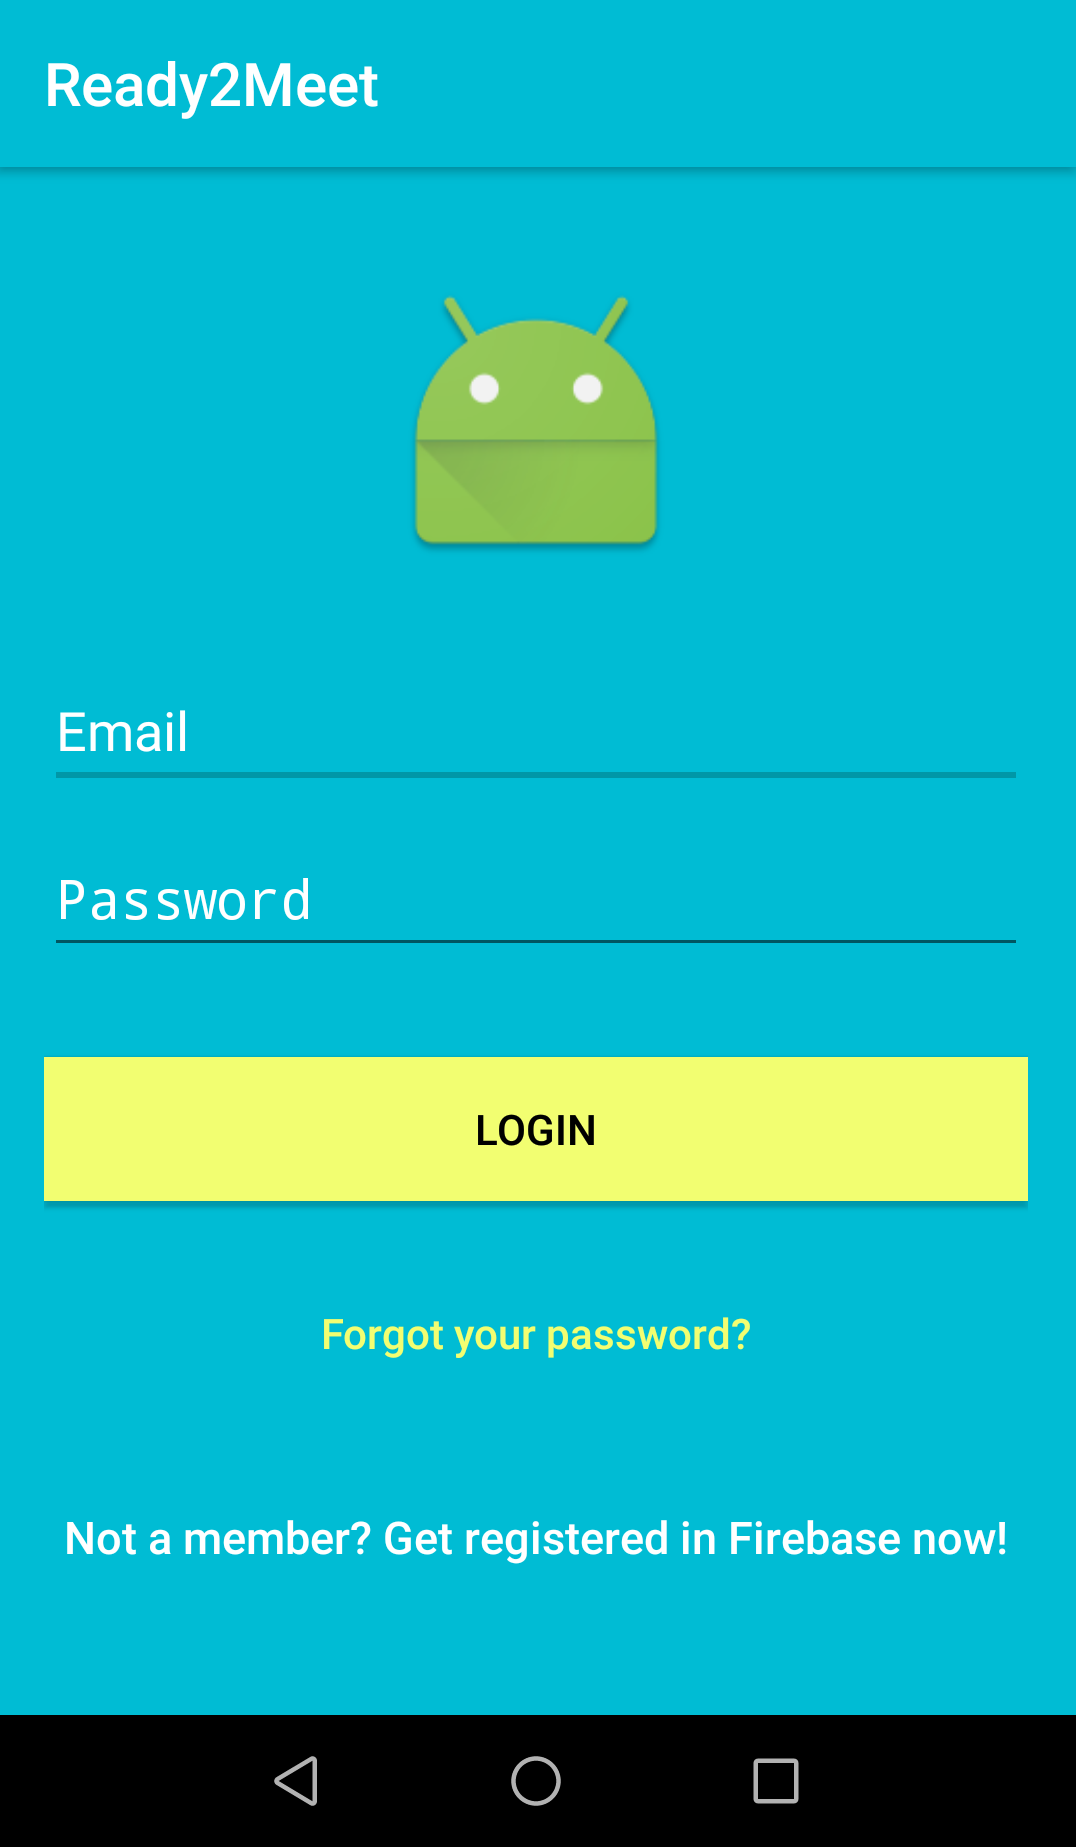
\includegraphics[height=0.85\textheight]{graphics/LoginScreen.png}}\qquad
    \subfloat[Start Screen]{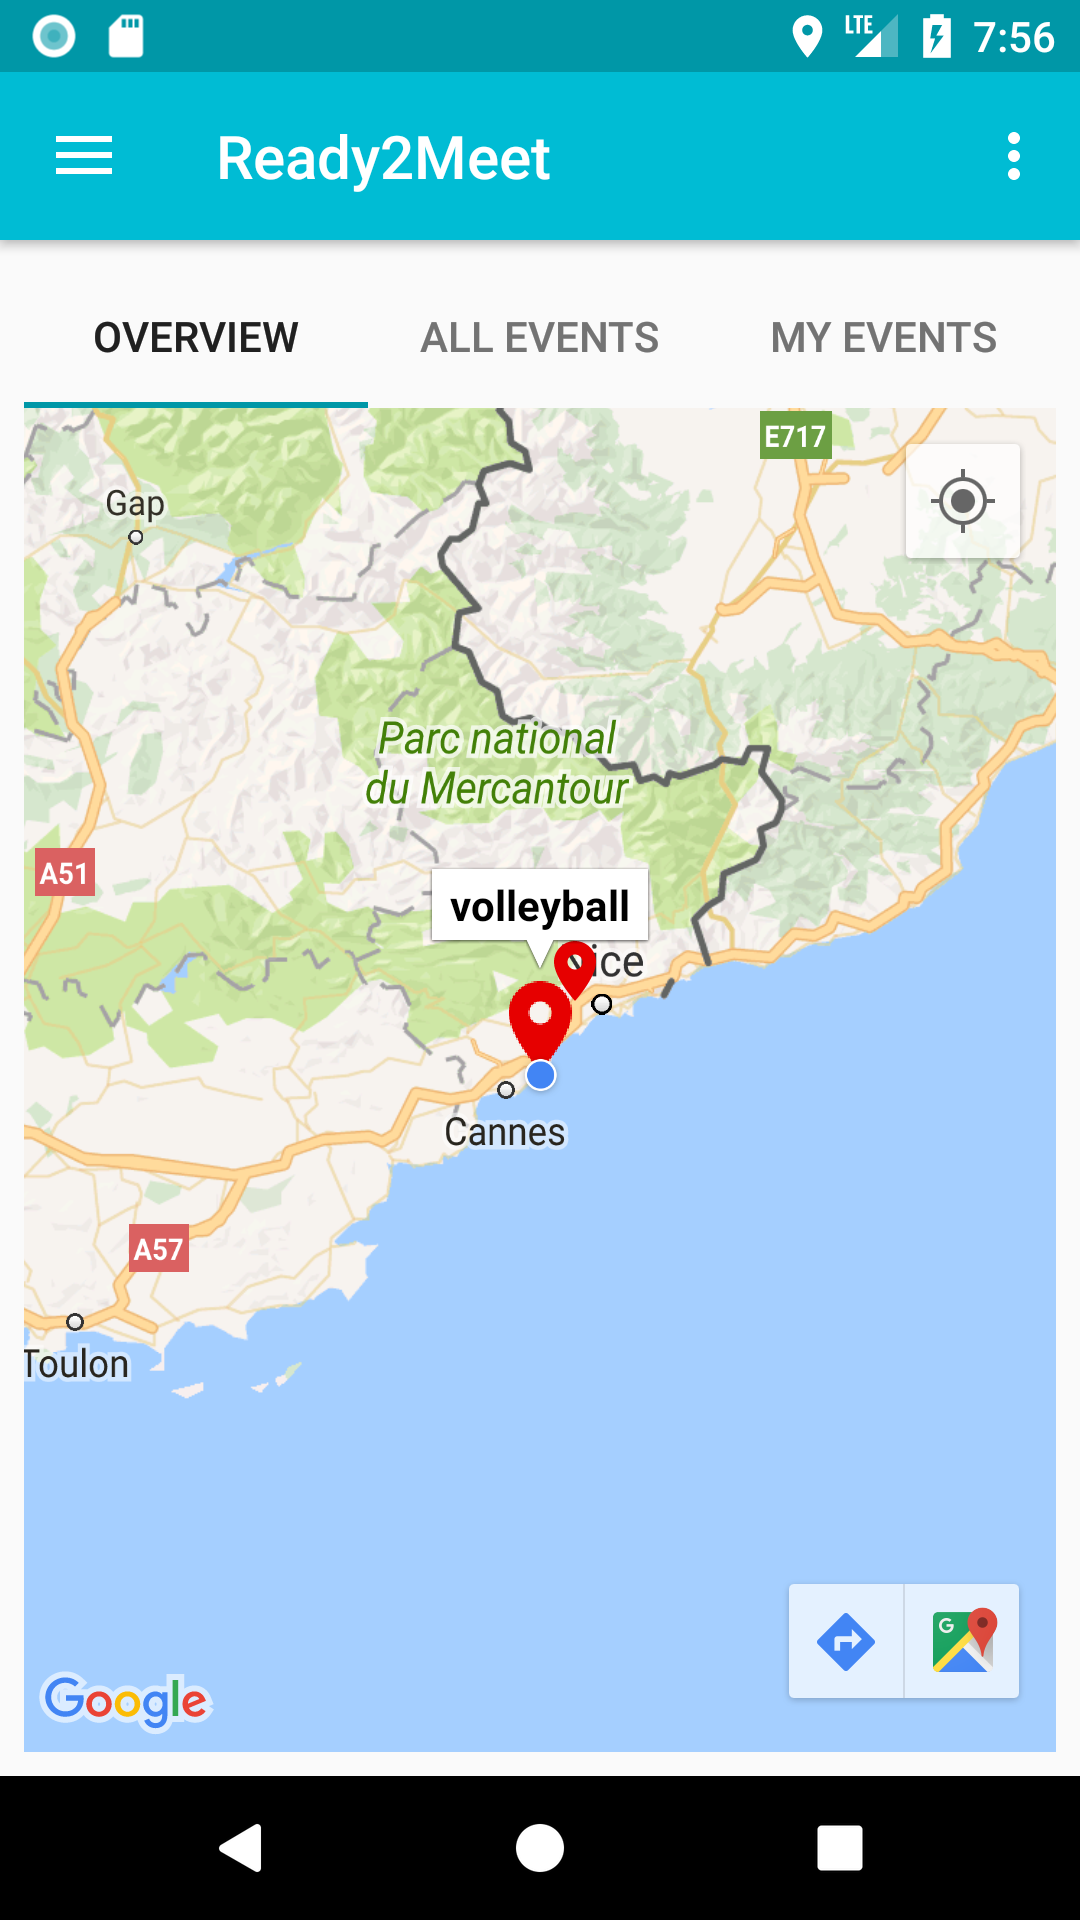
\includegraphics[height=0.85\textheight]{graphics/StartScreen.png}}
\end{figure}
\end{frame}

\begin{frame}{UI Design and Click Stream}
\begin{figure}
    \centering
    \subfloat[Event List]{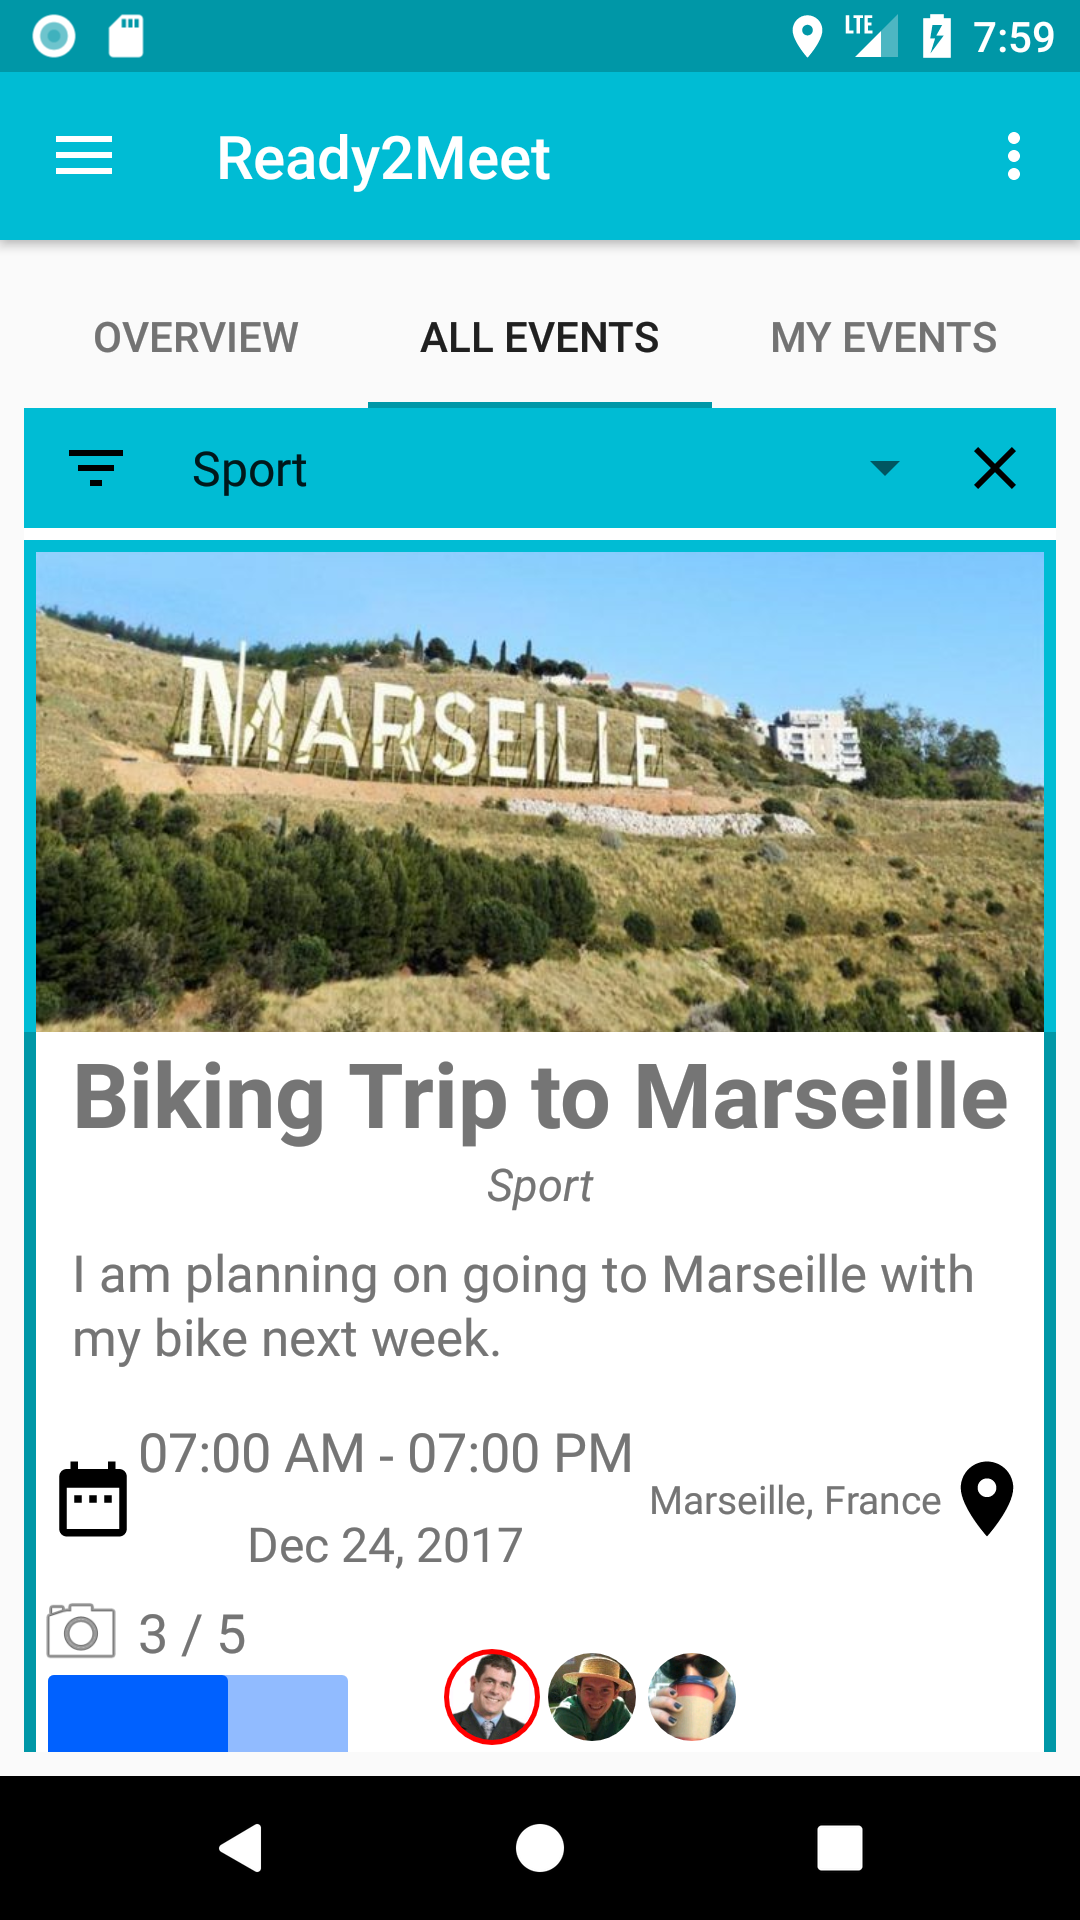
\includegraphics[height=0.85\textheight]{graphics/EventList.jpg}}\qquad
    \subfloat[Event Details]{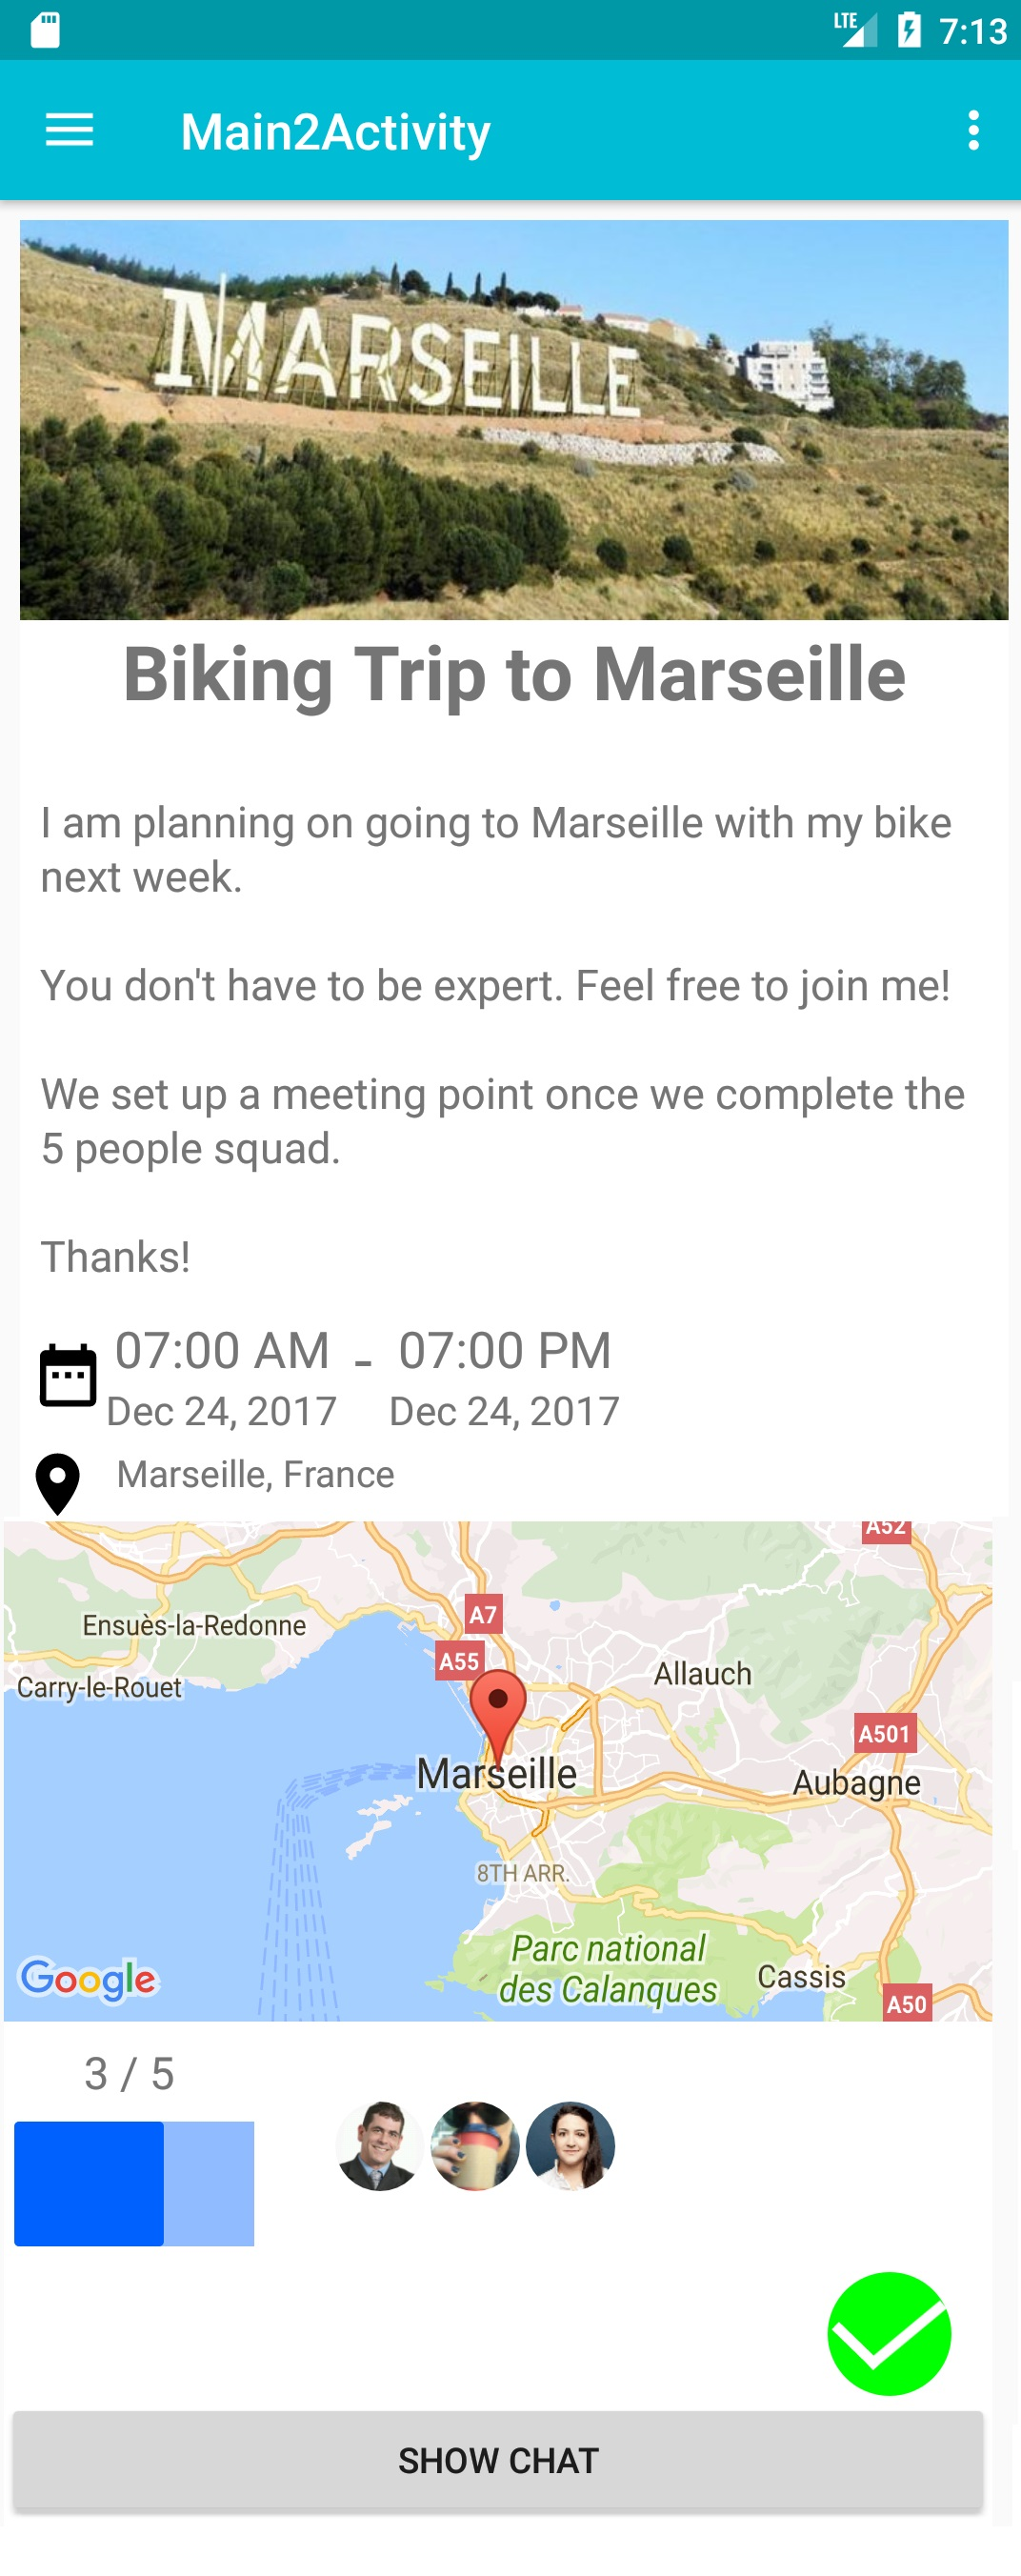
\includegraphics[height=0.85\textheight]{graphics/EventDetails.jpg}}
\end{figure}
\end{frame}

\begin{frame}{UI Design and Click Stream}
\begin{figure}
    \centering
    \subfloat[Chat]{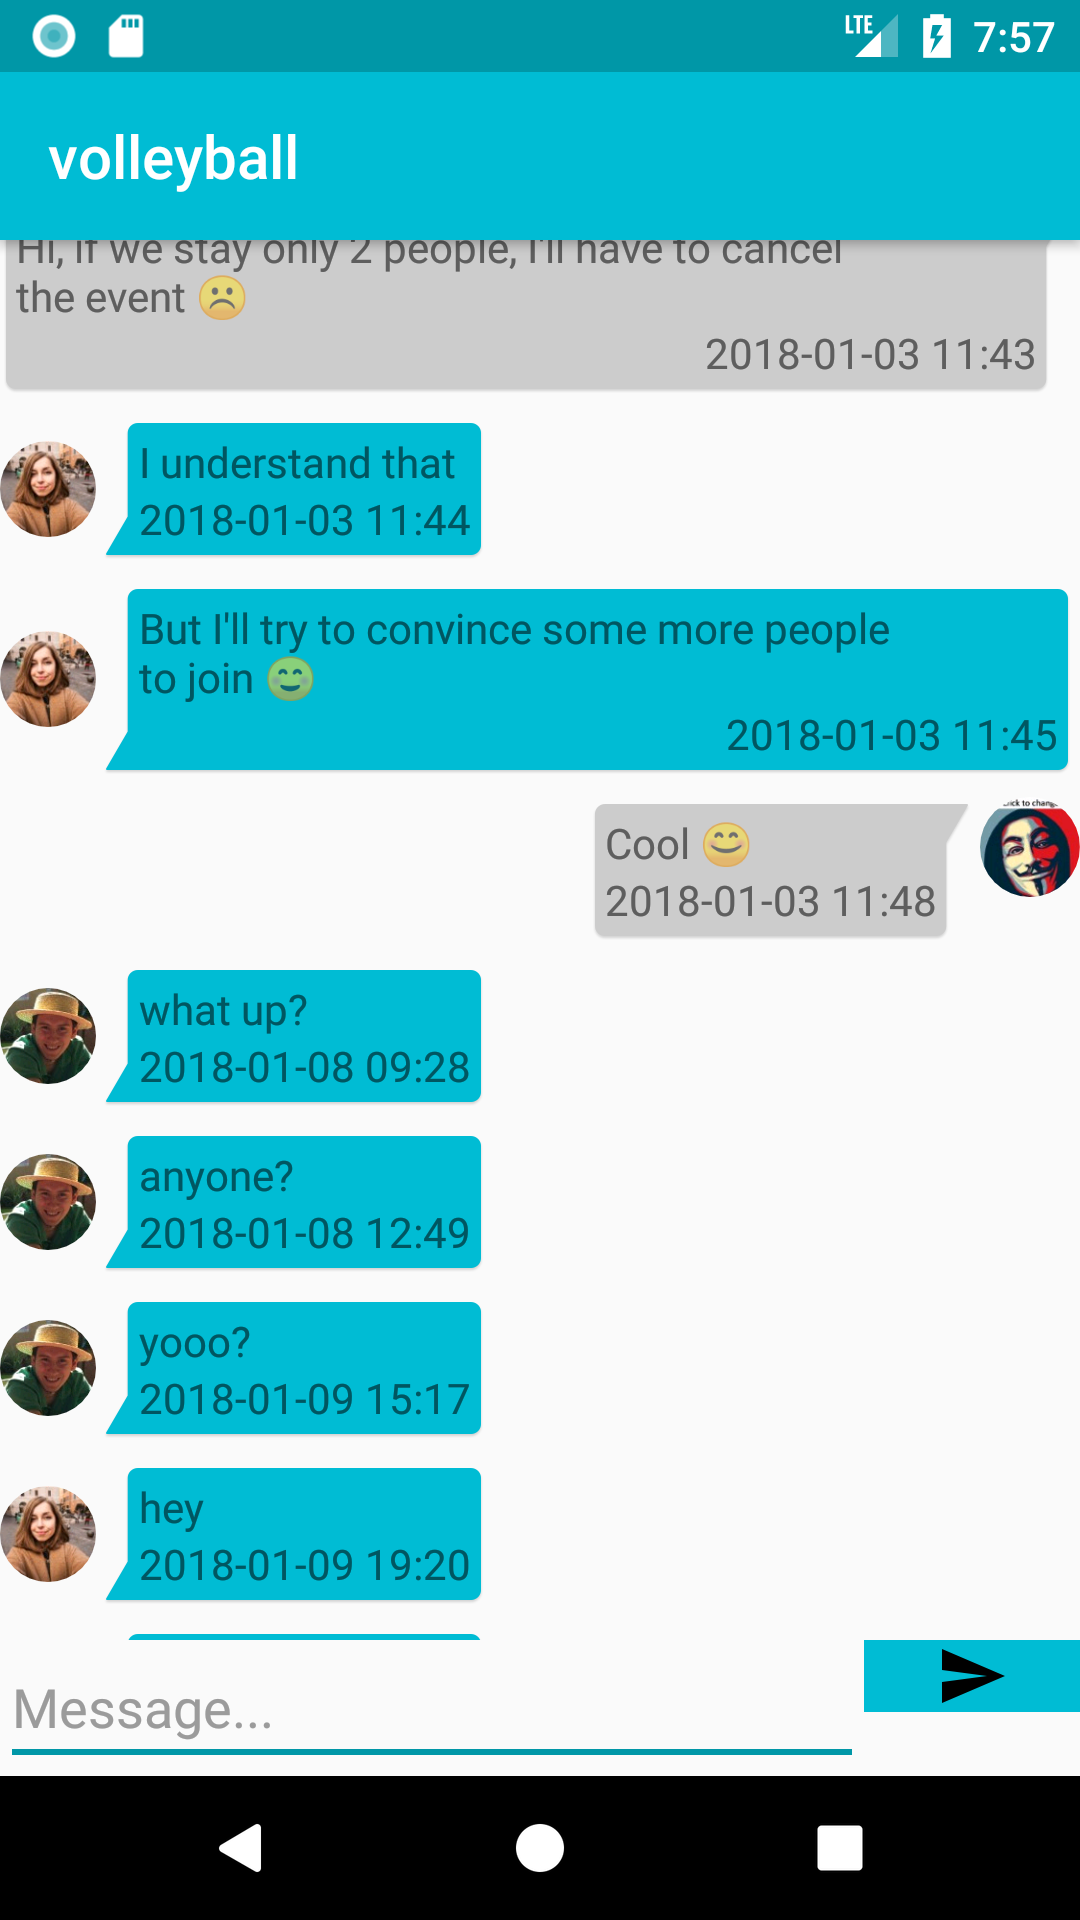
\includegraphics[height=0.85\textheight]{graphics/Chat.png}}\qquad
    \subfloat[Chat Notification]{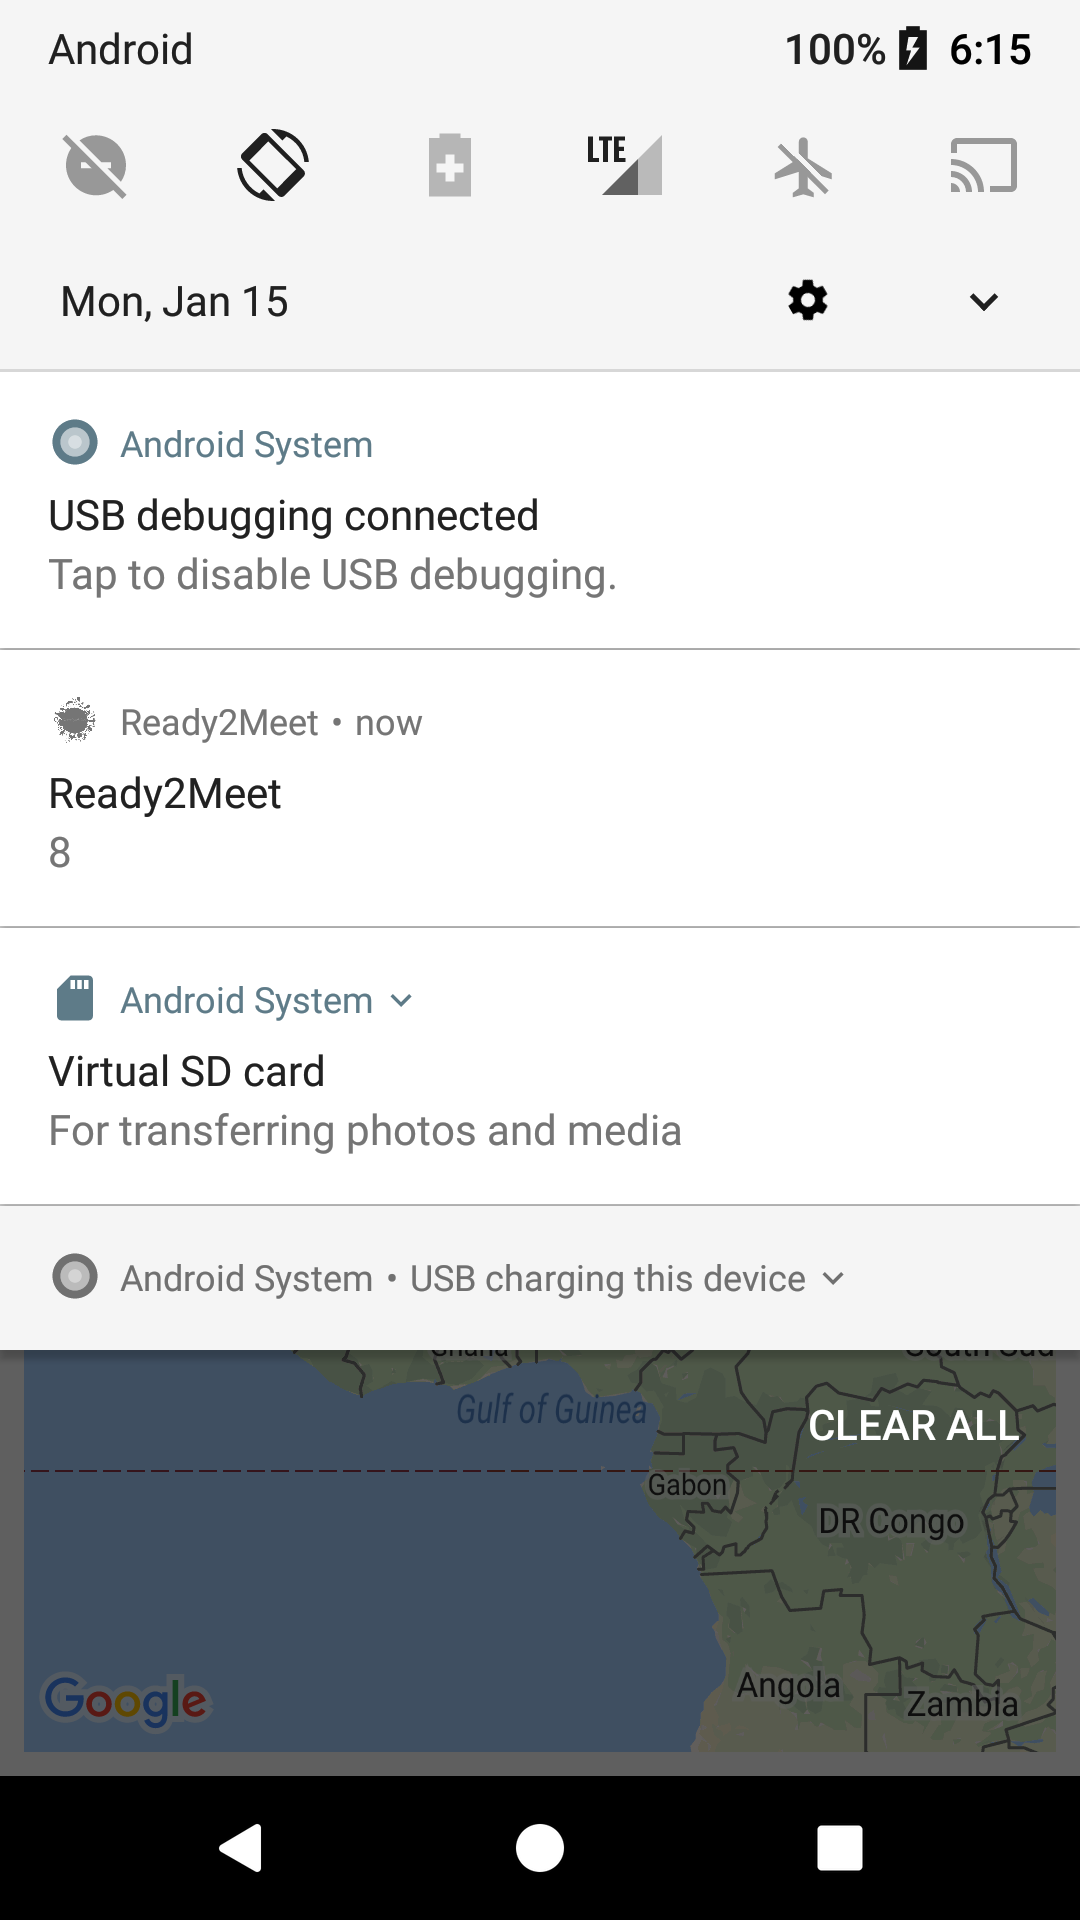
\includegraphics[height=0.85\textheight]{graphics/ChatNotification.png}}
\end{figure}
\end{frame}

\begin{frame}{UI Design and Click Stream}
\begin{figure}
    \centering
    \subfloat[Add Event]{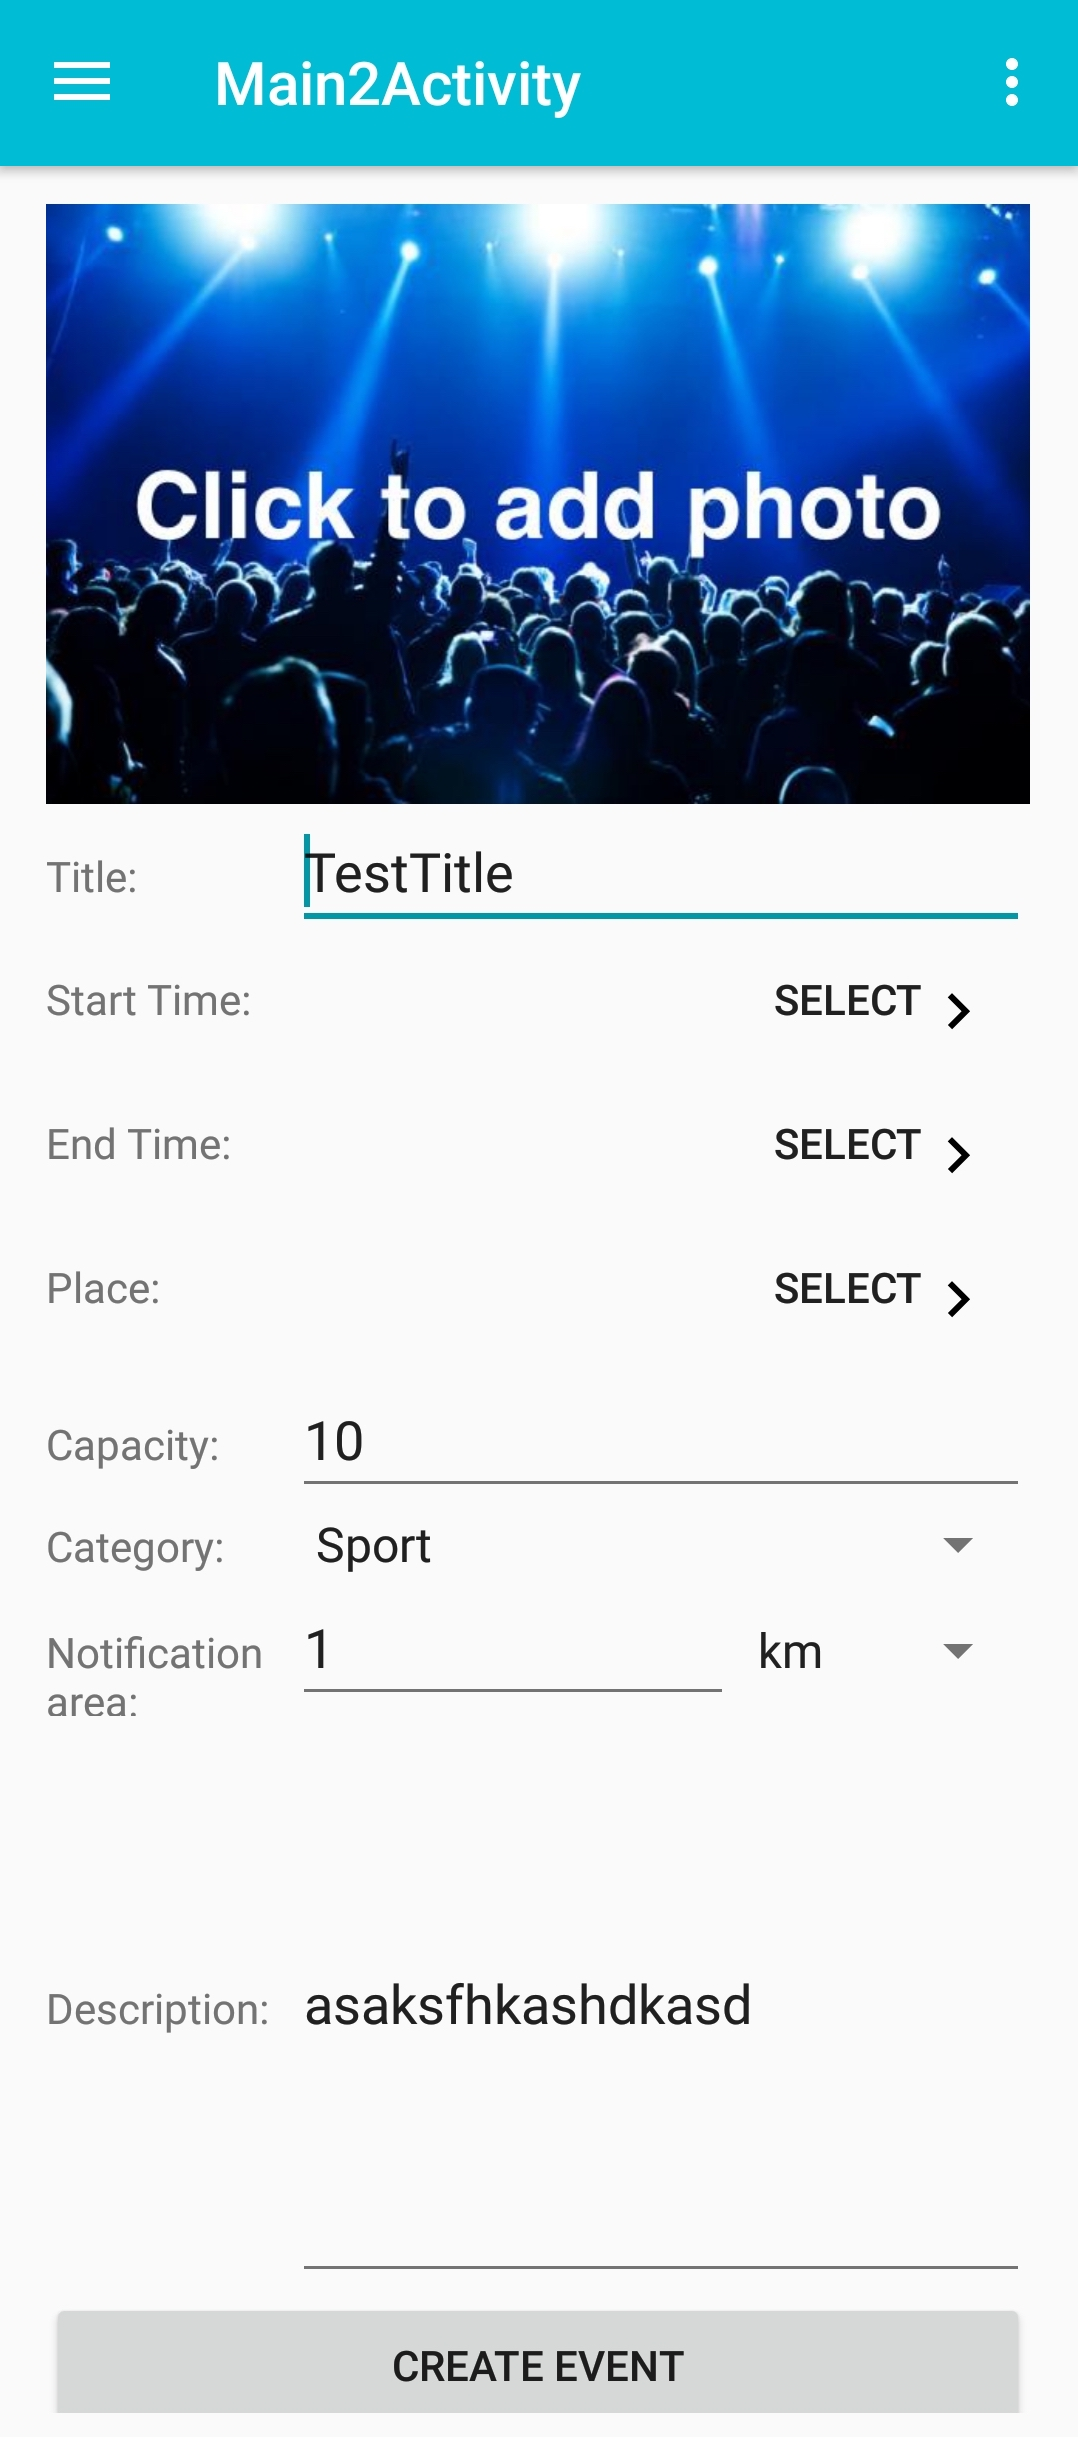
\includegraphics[height=0.85\textheight]{graphics/AddEvent.jpg}}\qquad
    \subfloat[Add Event Location]{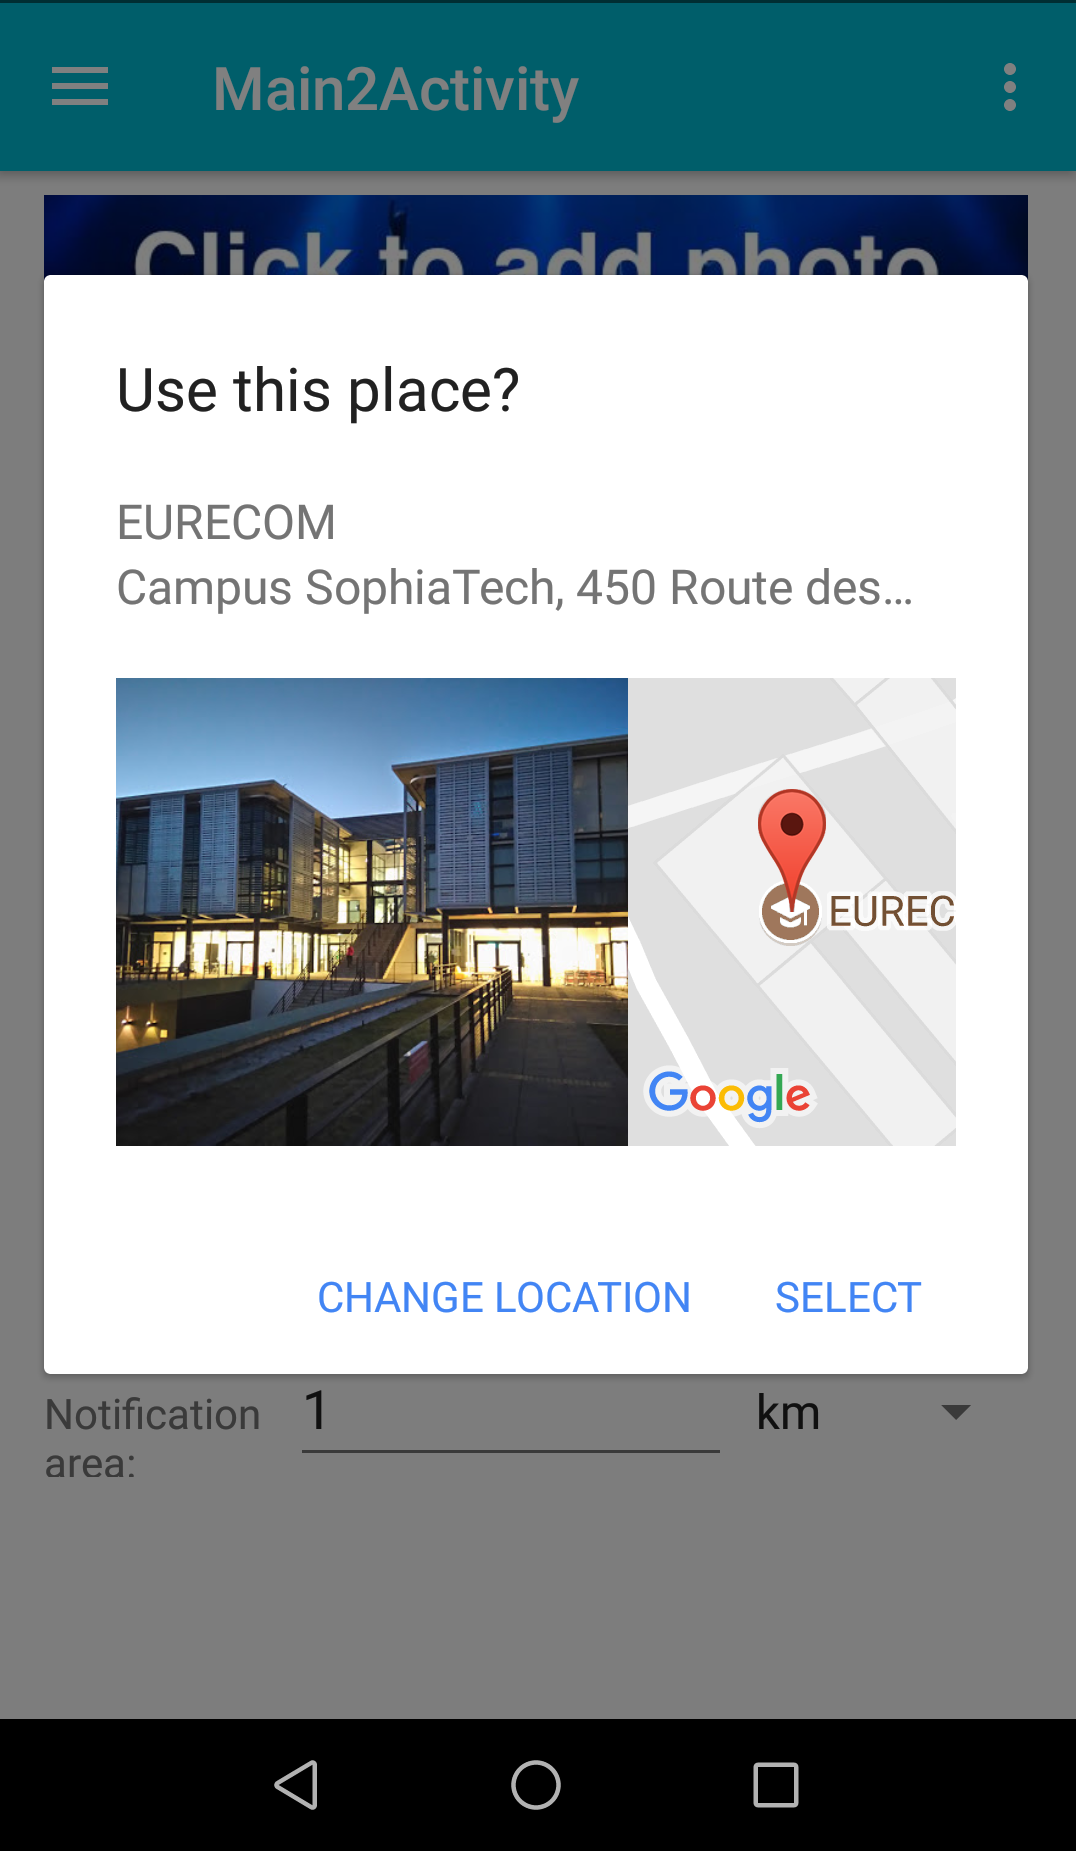
\includegraphics[height=0.85\textheight]{graphics/AddEvent_Location.png}}
\end{figure}
\end{frame}

\begin{frame}{Use Case -- Joining an event}
\begin{itemize}
\item User is in a new city (e.g. holidays) and wants to do something
\item User opens the app and sees events of different types nearby
\item User can join the event
\item During event: user can take and share pictures
\item In case of notifications: User is notified about new events or when his location changes
\end{itemize}
\end{frame}

\begin{frame}{Use Case -- Creating an event}
\begin{itemize}
\item User has an idea for an event
\item User opens the app and creates the event (time, place, category, capacity, \dots)
\item User can manage participants
\item Participants can organize themselves in a chatroom which is automatically created
\end{itemize}
\end{frame}

\begin{frame}{SW Architecture -- Database}
\begin{tikzpicture}[scale=0.6, every node/.style={scale=0.6}]
\umlclass{fr.eurecom.Ready2Meet.database::User}{
+ DisplayName : String\\
+ ParticipatingEvents: Map\textless String, Boolean\textgreater\\
+ ProfilePictureURL : String
}{} (User);

\umlclass[right of=User, node distance=10cm]{fr.eurecom.Ready2Meet.database::Message}{
+ message : String\\
+ senderId : String\\
+ time : String
}{};
\end{tikzpicture}\bigskip

\begin{tikzpicture}[scale=0.6, every node/.style={scale=0.6}]
\umlclass{fr.eurecom.Ready2Meet.database::Event}{
+ id : String\\
+ title : String\\
+ description : String\\
+ owner : String\\
+ current : Long\\
+ categories : Map\textless String, Boolean\textgreater\\
+ capacity : Long\\
+ picture : String\\
+ place : String\\
+ startTime : String\\
+ endTime : String\\
+ Participants : Map\textless String, Boolean\textgreater\\
%+ WhoReported Map\textless String, Boolean\textgreater\\
+ notificationArea : Long\\
+ latitude : Double\\
+ longitude : Double
}{}
\end{tikzpicture}
\end{frame}

\begin{frame}{SW Architecture -- Activities}
% http://perso.ensta-paristech.fr/~kielbasi/tikzuml/var/files/doc/tikzumlmanual.pdf
\begin{tikzpicture}[scale=0.6, every node/.style={scale=0.6}]
\umlsimpleclass{AppCompatActivity}
\umlsimpleclass[type=interface, x=8]{OnNavigationItemSelectedListener}
\umlsimpleclass[type=abstract, x=11.3, y=-3]{ToolbarActivity}
\umlsimpleclass[x=-2, y=-3]{ResetPasswordActivity}
\umlsimpleclass[x=2, y=-3]{SignupActivity}
\umlsimpleclass[x=5.3, y=-3]{LoginActivity}
\umlsimpleclass[x=8.3, y=-3]{ChatActivity}
\umlsimpleclass[x=11.3, y=-6]{MainActivity}
\umlsimpleclass[x=8, y=-6]{AddEventActivity}

\umlimpl{ToolbarActivity}{OnNavigationItemSelectedListener}
\umlVHVinherit{ToolbarActivity}{AppCompatActivity}
\umlVHVinherit{MainActivity}{ToolbarActivity}
\umlVHVinherit{AddEventActivity}{ToolbarActivity}
\umlVHVinherit{LoginActivity}{AppCompatActivity}
\umlVHVinherit{ChatActivity}{AppCompatActivity}
\umlVHVinherit{SignupActivity}{AppCompatActivity}
\umlVHVinherit{ResetPasswordActivity}{AppCompatActivity}
\end{tikzpicture}
\end{frame}

\begin{frame}{SW Architecture -- Fragments}
\begin{tikzpicture}[scale=0.6, every node/.style={scale=0.6}]
\umlsimpleclass[type=interface, x=-5]{OnMapReadyCallback}
\umlsimpleclass[x=2]{Fragment}
\umlsimpleclass[x = -4, y=-3]{EventDetailFragment}
\umlsimpleclass[y=-3]{AllEvents}
\umlsimpleclass[x = 4, y=-3]{DashboardFragment}
\umlsimpleclass[x = 8, y=-3]{AccountOptions}

\umlimpl{EventDetailFragment}{OnMapReadyCallback}
\umlimpl{DashboardFragment}{OnMapReadyCallback}
\umlVHVinherit{EventDetailFragment}{Fragment}
\umlVHVinherit{AllEvents}{Fragment}
\umlVHVinherit{DashboardFragment}{Fragment}
\umlVHVinherit{AccountOptions}{Fragment}
\end{tikzpicture}
\end{frame}

\begin{frame}{SW Architecture -- Services}
\begin{figure}
\centering
\begin{tikzpicture}[scale=0.6, every node/.style={scale=0.6}]
\umlsimpleclass[x=5]{FirebaseMessagingService}
\umlsimpleclass[x = 5, y=-3]{ChatNotificationService}
\umlsimpleclass[x = 11]{FirebaseInstanceIdService}
\umlsimpleclass[x = 11, y=-3]{MyFirebaseInstanceIdService}

\umlVHVinherit{MyFirebaseInstanceIdService}{FirebaseInstanceIdService}
\umlVHVinherit{ChatNotificationService}{FirebaseMessagingService}
\end{tikzpicture}
\end{figure}
\end{frame}

\begin{frame}{SW Architecture -- Fragments}
\begin{figure}
\centering
\begin{tikzpicture}[scale=0.6, every node/.style={scale=0.6}]
\umlsimpleclass[type=interface, x=-5]{OnMapReadyCallback}
\umlsimpleclass[x=2]{Fragment}
\umlsimpleclass[x = -4, y=-3]{EventDetailFragment}
\umlsimpleclass[y=-3]{AllEvents}
\umlsimpleclass[x = 4, y=-3]{DashboardFragment}
\umlsimpleclass[x = 8, y=-3]{AccountOptions}

\umlimpl{EventDetailFragment}{OnMapReadyCallback}
\umlVHVinherit{EventDetailFragment}{Fragment}
\umlVHVinherit{AllEvents}{Fragment}
\umlVHVinherit{DashboardFragment}{Fragment}
\umlVHVinherit{AccountOptions}{Fragment}
\end{tikzpicture}
\end{figure}
\end{frame}

\begin{frame}{Interaction with Backend}
\begin{figure}
\centering
\begin{tikzpicture}
\node[inner sep=0pt] (ANDROID) at (0,1.5) {
\includegraphics[width=.07\textwidth]{graphics/android.jpg}};
\node[inner sep=0pt] (FIREBASE) at (6,1.5) {\includegraphics[width=.1\textwidth]{graphics/firebase.png}};

\draw[thick] (0,1) -- (0,-5);
\draw[thick] (6,1) -- (6,-5);

\node at (-1, 0.7) {Add Event};
\draw[thick,->] (0, 0.5) -- (6, 0.5) node[midway, above] {Add Event};

\node at (-1, -0.7) {Join Event};
\draw[thick,->] (0, -1) -- (6, -1) node[midway, above] {Add User to Event Participants};

\node at (-1.3, -2.2) {Send Message};
\draw[thick,->] (0, -2.5) -- (6, -2.5) node[midway, above] {Add Message};

\node[inner sep=0pt] at (8, -1.0) {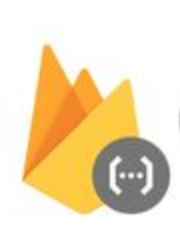
\includegraphics[width=.1\textwidth]{graphics/CloudFunctions.png}};
\draw[thick] (8, -1.6) -- (8,-5);
\draw[thick,->] (6, -3.2) -- (8, -3.2) node[midway, above] {New Message};
\draw[thick,->] (8, -3.8) -- (6, -3.8) node[midway, above] {Get Users};
\draw[thick,->] (8, -4.3) -- (0, -4.3) node[midway, above] {Send Notification};

\end{tikzpicture}
\end{figure}
\end{frame}

\begin{frame}{Technical Details}
Permissions:
\begin{itemize}
\item Internet
\item Location
\item Read and write calendar\bigskip
\end{itemize}
Frameworks used:
\begin{itemize}
\item Firebase: Realtime database
\item Picasso/Glide: Image rendering
\item Google Play Services: Maps/Places
\item UI: RoundCornerProgressBar, circleimageview, customcheckbox
\end{itemize}
\end{frame}

\begin{frame}{Status and Planning -- SW development methodology}
\begin{itemize}
\item Git (repo: \url{https://github.com/KuechA/mobEvent})
\item Agile development using 2 techniques:
	\begin{itemize}
	\item Rapid application development: Prototyping, Adjustment of requirements
	\item Chaos model: Resolve most important issue first
	\end{itemize}
\item Continuous discussion about own task attributions, issues etc. via WhatsApp
\end{itemize}
\end{frame}

\begin{frame}{Status and Planning -- Project status}
\begin{itemize}
\item Creating and joining events
\item Real-time information for the user
\item User-preferences taken into account
\item Interaction with calendar
\item Photo gallery for each event
\item Chat for each event (incl. notifications)
\end{itemize}
\end{frame}

\begin{frame}{Status and Planning -- Task attribution}
\begin{itemize}
\item Berkay:
	\begin{itemize}
	\item User management
	\item Event list
	\item UI enhancements
	\item Support with event details
	\end{itemize}
\item Alex:
	\begin{itemize}
	\item Adding events
	\item Chat
	\item Landing page
	\item Event details
	\item Backend (Firebase functions)
	\item UI improvements
	\end{itemize}
\item Saad: UI
\end{itemize}
\end{frame}

\begin{frame}
\centering{\textcolor{EURECOMblue}{\Huge{DEMO}}}
\end{frame}

\begin{frame}
\centering{\textcolor{EURECOMblue}{\Huge{Questions?}}}
\end{frame}

\end{document}
